\subsection{M.PD.11 - Code coverage}

\begin{figure}[H]
  \centering
  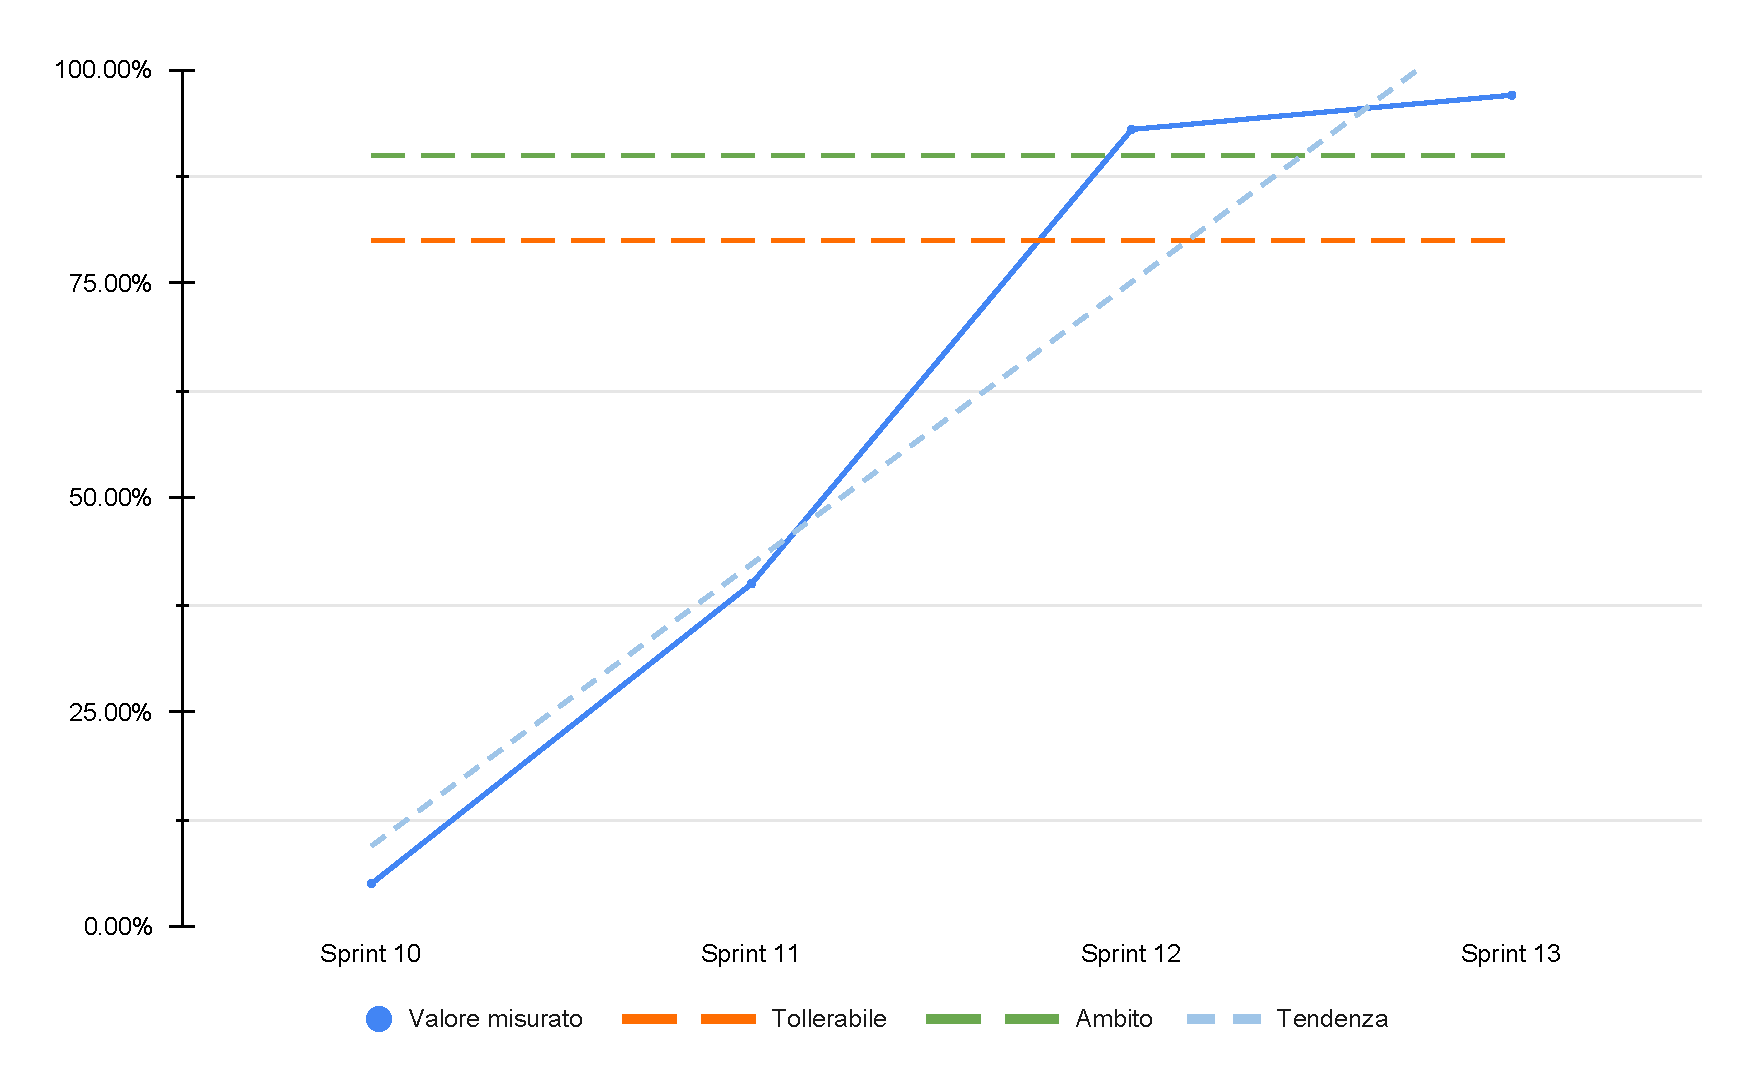
\includegraphics[width=\textwidth]{assets/code_coverage.pdf}
  \caption{M.PD.11 - Code coverage}
\end{figure}

\par Nei primi due sprint della \glossario{PB}, la maggior parte delle risorse è stata dedicata alla scelta del modello architetturale e alla progettazione del software. Di conseguenza, il team ha dato priorità alla codifica, concentrandosi sulla definizione di una struttura solida per il codice sorgente. Durante la seconda metà dello \glossario{sprint} 11, il gruppo ha riscontrato difficoltà nella configurazione dell'ambiente di test; questo ha ostacolato l'esecuzione parallela delle attività di codifica e testing. Nonostante ciò, il team ha organizzato incontri per approfondire l'uso degli strumenti di testing, al fine di avviare i test con il minor ritardo possibile. Tale approccio ha permesso al gruppo di implementare un buon numero di test sia per il \glossario{front-end} che per il \glossario{back-end} entro la fine dello sprint 11. A partire dal dodicesimo sprint, le attività di codifica e testing sono state svolte in parallelo, raggiungendo una copertura del codice superiore al valore ambito.